\begin{justifying}
  \noindent 
  Hasta ahora no hemos abordado el cambio. Pero, si creemos en la ciencia, debemos defender el postulado ontológico de que todo 
  está en constante cambio. De hecho, las ciencias describen, explican, predicen, 
  controlan o provocan cambios de diversos tipos, como el movimiento, la acreción, 
  la división y la evolución. Por lo tanto, la ontología debería analizar y sistema tizar estos diversos tipos de cambio.
  Mientras algunos metafísicos se han dedicado a elogiar el cambio, otros lo han negado y ninguno lo ha descrito correctamente. Nos esforzaremos por construir un concepto de cambio lo suficientemente amplio y, por lo tanto, lo suficientemente pobre como para abarcar todos los conceptos de cambio, en particular los que se dan en las ciencias, y esbozar teorías generales del cambio de algunos tipos típicos. Estos son los objetivos del presente capítulo, dedicado al cambio en general. El tema del cambio cualitativo se abordará en el volumen complementario, \textit{Un Mundo de Sistemas}.
  Un cambio es un evento o un proceso, ya sea cuantitativo, cualitativo o ambos. Sea cual sea su naturaleza, un cambio es una modificación en o de alguna cosa o cosas: más precisamente, consiste en una variación del estado de una entidad. Dicho de forma negativa, no existe cambio separado de las cosas; ni, de hecho, existen cosas inmutables, aunque algunas cambien lentamente o solo en ciertos aspectos limitados. El mundo, entonces, consiste en cosas que no permanecen en el mismo estado para siempre. Esta hipótesis metafísica es una extrapolación tanto de la experiencia ordinaria como del conocimiento científico. La hipótesis contraria, que nada cambia, es una extravagancia filosófica poco digna de la consideración de una persona cuerda.

  \newpage

	\noindent Conocimiento de la naturaleza de la cosa en cuestión: por lo tanto,
	es idealmente adecuado para la ontología o la teoría general de las cosas.
	Comencemos entonces recordando brevemente las nociones de estado y espacio de estados,
	para adentrarnos inmediatamente al fondo del asunto.

	\section{\centering \large CAMBIABILIDAD}
	\subsection{Preliminares}
	\noindent Todo se encuentra en un estado u otro en relación con un marco de referencia determinado.
	Y cada estado (relativo) de una cosa viene determinado de forma única por las
	propiedades de esta última (en relación con algún marco). Por lo tanto, el estado de una cosa
	con n propiedades, cada una representada por una función (de estado), es una n-tupla de
	valores de las funciones que representan esas propiedades. Los diferentes estados
	corresponden a (están representados por) diferentes n-tuplas. Un cambio en la
	representación de las propiedades, o en la elección del marco de referencia, da lugar a
	una representación diferente de los estados. Esto demuestra que nuestro conocimiento de
	un estado depende en parte de nosotros mismos y del estado de la técnica, pero no
	de que el estado en sí mismo sea un artefacto del observador. En resumen, los estados
	son relativos.

	Supongamos, para mayor precisión, que un objeto x, como el obturador de una cámara o un interruptor 
    eléctrico, tiene una única propiedad general dicotómica: que está abierto (1) o cerrado (0). 
    Los posibles estados de x son entonces 0 y 1. En otras palabras, el espacio de estados de x es S(x)={O, I}.
    En realidad, esto es una simplificación excesiva: 0 y 1 son solo los estados de interés para algunos propósitos 
    específicos. Cualquier objeto real tiene un gran número n de propiedades Pi', cada una representable por una función Fj, donde 1 ~ i ~ n.
    Los posibles grados o intensidades de la propiedad Pi se representan como tantos valores de la función Fj. 
    Por lo tanto, el espacio de estados concebible del objeto será el producto vectorial de las imágenes de estas funciones. 
    Y el espacio de estados nomológico será un subconjunto del espacio anterior, resultante de las leyes que involucran a Pi: 
    véase la Figura 5.1. Todo esto es válido, por supuesto, para una representación dada de propiedades, y por tanto de estados.


	\begin{center}
		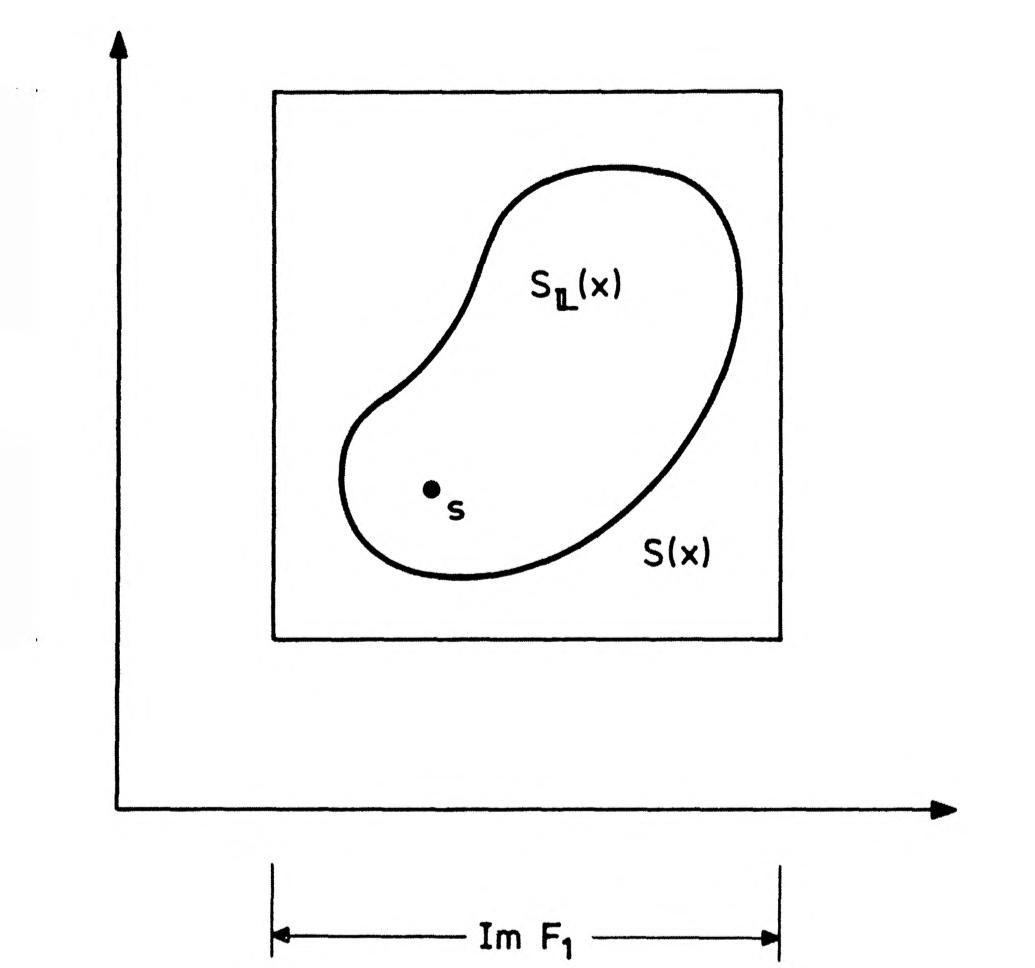
\includegraphics[width=0.6\textwidth]{img/Figura5-1.png}
		\\ \scriptsize Fig. 5.l. El espacio de estados concebible $S(x)$ y el espacio de estados legítimo $S_\mathrm{L}(x)$ de una cosa $x$
		con dos propiedades representadas por las funciones $F_\mathrm{1}$ y $F_\mathrm{2}$.
		\textit{'$F$'} se lee \textit{'la imagen $F$'} es el conjunto de valores, o rango, de $F$.
	\end{center}


	\noindent la curva con la ayuda de un parámetro, cuya interpretación estándar es el tiempo.
	Pero una de las ventajas de la representación del cambio en el espacio de estados
	es que no requiere el uso explícito del concepto de tiempo.

	Para aclarar las ideas, consideremos el espacio de estados del conjunto genético de una población
	de organismos. Ese conjunto está incluido en el espacio cartesiano cuyos ejes son
	las frecuencias genéticas del conjunto. Cada punto de este espacio representa un estado posible del conjunto genético. El punto representativo, el que representa el estado real del sistema, permanecerá fijo solo si los organismos no sufren mutaciones, lo que nunca ocurre, ni siquiera si el entorno de la población es muy estable, como una laguna tropical.
	De lo contrario, el punto representativo se mueve (en el espacio de estados, no en el espacio ordinario) describiendo una trayectoria. Esta curva, que en el caso de la evolución biológica no tiene bucles, representa la historia genética del conjunto genético.
	De lo contrario, el punto representativo se mueve (en el espacio de estados, no en el espacio ordinario)
	describiendo una trayectoria. Esta curva, que en el caso de la
	evolución biológica no tiene bucles , representa la historia genética del
	pool genético, o la evolución de la población correspondiente a nivel genético.
	Cualquier segmento de la historia total puede denominarse evento o
	proceso que involucra al pool genético. (Véase la figura 5.2).

	\begin{center}
		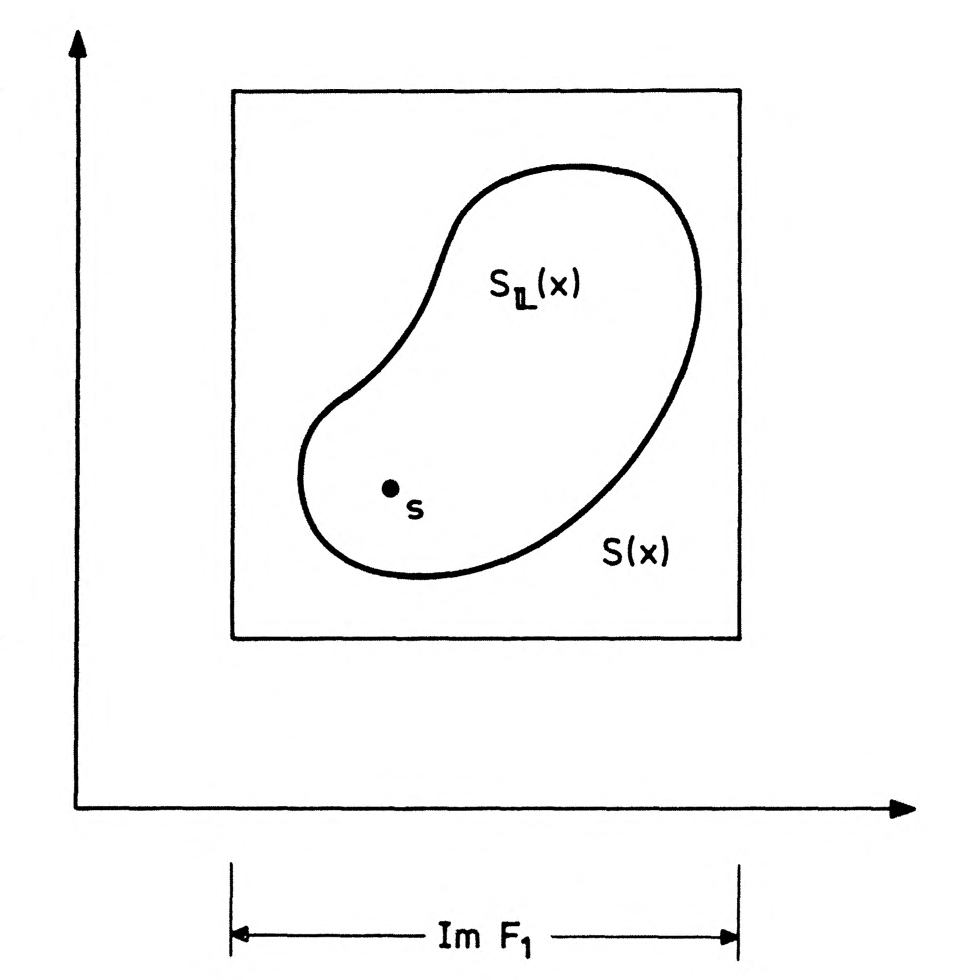
\includegraphics[width=0.6\textwidth]{img/Figura5-2.png}
		\\ \scriptsize Fig. 5.2. El cambio en las frecuencias genéticas en un acervo genético,
		en respuesta a la acción conjunta de la mutación y la selección.
		Los extremos de la curva representan el origen y la extinción de la población dada.
	\end{center}
    Demasiado para un trasfondo intuitivo.

    \subsection{Capacidad de cambio}
    \noindent Antes de abordar el cambio real, conviene aclarar la noción intuitiva
    de mutabilidad o variabilidad:

    \bigskip

    \noindent DEFINICIÓN 5.1: Sea $x$ una cosa. Entonces
    \begin{enumerate}[label=(\roman*), itemsep=0pt, parsep=0pt]
        \item $x$ es inmutable si y solo si $S_\mathrm{L}(x)$ es un singleton para todas las elecciones de función de estado para $x$.
        \item $x$ es cambiante (o mutable) si y solo si $S_\mathrm{L}(x)$ tiene al menos dos miembros distintos
            para todas las elecciones de función de estado para $x$.
    \end{enumerate}

    \bigskip

    \noindent POSTULADO 5.1 Toda cosa (concreta) tiene al menos dos estados distintos y 
    el espacio de estados de cualquier construcción está vacío. Es decir:
    \begin{enumerate}[label=(\roman*), itemsep=0pt, parsep=0pt]
        \item si $x$ es una cosa, entonces, para todas las elecciones de la función de estado para $x$, $|S_\mathrm{L}(x)| \geq 2$.
        \item si y es una construcción, entonces no hay funciones de estado para $y$, $o$, equivalentemente, $S_\mathrm{L}(y) = \varnothing$.
    \end{enumerate}

    Una consecuencia inmediata del Postulado 5.1 y la Definición 5.1 es

    \bigskip

    \noindent COROLARIO 5.1 Todas las cosas (concretas) son cambiantes, y las construcciones
    no son ni inmutables ni cambiantes.

    Observación 1. No estamos afirmando (todavía) que todo esté realmente
    sufriendo algún tipo de cambio, sino solo que puede cambiar. Observación
    2. La segunda parte del Corolario 5.1 afirma que las categorías de cambio
    e inmutabilidad no se aplican a los constructos. Los constructos no son ni
    objetos eternos (Platón) ni cambiantes (Hegel). Lo que cambia
    de una persona a otra son los procesos cerebrales que se producen cuando se piensan los constructos. \\
	Nuestro siguiente concepto es el del cambio global, independientemente del orden en que se produzca:

    \bigskip

    \noindent DEFINICIÓN 5.2 Sea $S_\mathrm{L}(x)$ un espacio de estados legítimo de una cosa $x$, y sean $S_\mathrm{i}(x)$, 
    $S_\mathrm{j}(x) \subset S_\mathrm{L}(x)$ dos colecciones de estados de $x$ [por ejemplo, dos regiones de
    $S_\mathrm{L}(x)$]. Entonces, el cambio global de $x$ entre $S_\mathrm{i}(x)$ y$S_\mathrm{i}(x)$ es igual a la
    diferencia simétrica entre los subconjuntos dados:

	\medskip

	$X_\mathrm{ij}(x) \:= \:S_\mathrm{i}(x) \:\triangle \: S_\mathrm{j}(x)$.

	\medskip

	Un cambio general puede ser leve o grande, superficial o profundo. Si
	hay cambios considerables en las propiedades individuales de una cosa, pero la
	cosa no adquiere ni pierde ninguna propiedad general, podemos decir que
	sufre un gran cambio. Si, por el contrario, una cosa gana o pierde
	propiedades generales, entonces se puede decir que sufre un cambio profundo.
	Mientras que en el primer caso los ejes del espacio de estados permanecen fijos, en el
	segundo se añaden o se eliminan algunos. Obtenemos una descripción fluida de
	este tipo de cambio si construimos el espacio de estados con todos los ejes necesarios
	y utilizamos en cada momento solo aquellas partes del espacio total que
	se refieren a las propiedades que realmente posee la cosa en ese momento. En la
	figura 5.3 representamos la evolución de una cosa imaginaria que sufre un
	cambio profundo. La primera parte del proceso se describe mediante una curva en el
	plano horizontal $lm \: F_\mathrm{1} \times lm \: F_\mathrm{2}$; la segunda parte se describe mediante una curva
	en el plano vertical. El cambio cualitativo se produce en la
	unión de las dos curvas. Toda la curva es continua, aunque
	su tangente tenga una discontinuidad.

	\bigskip

	\begin{center}
		\title{\normalsize CAPITULO 5}
	\end{center}

	\smallskip

	\begin{center}
		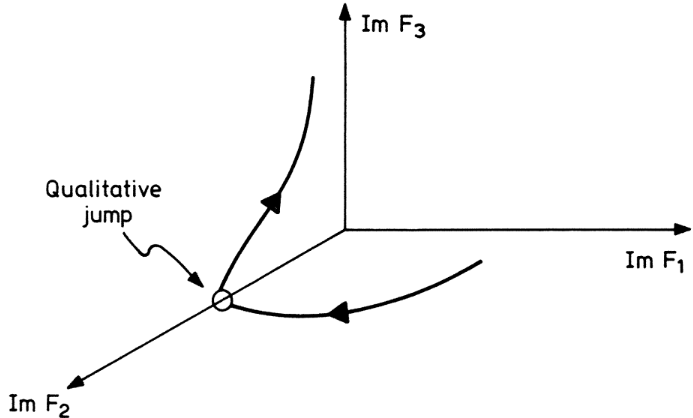
\includegraphics[width=0.7\textwidth]{img/Figura5-3.png}
		\\ \scriptsize Fig. 5.3. Cada arco de la curva describe un cambio cuantitativo. 
		Un salto cualitativo ocurre en la unión de los dos arcos.
	\end{center}

	\bigskip

	En otras palabras, adoptamos

	\bigskip

	\noindent DEFINICIÓN 5.3 Sea $\mathbb{F}$ una función de estado que abarca todo el espacio de estados
	$S_\mathrm{L}(x)$ para una cosa $x$. La cosa sufre un \textit{cambio cualitativo} si y solo si
	$S_\mathrm{L}(x)$ es igual a la unión de al menos dos subespacios, cada uno de los cuales está
	abarcado por una proyección diferente de $\mathbb{F}$. De lo contrario [es decir, si ninguno de los
	componentes puede ignorarse durante ninguna parte del proceso], la cosa
	solo sufre un \textit{cambio cuantitativo}.

	Una consecuencia inmediata de esta definición es

	\bigskip

	COROLARIO 5.2 Todo cambio cualitativo va acompañado de un cambio cuantitativo.
	[Es decir, para cualquier cosa $x$, si $x$ cambia cualitativamente, entonces $x$ cambia cuantitativamente].

	Lo contrario no se cumple, lo cual es mejor, ya que es falso.
	Tenga en cuenta que lo anterior no es una hipótesis ontológica independiente, sino un
	mero corolario de una convención. El problema es que esta última se ha
	formulado de manera que se obtenga esa consecuencia.

	Hasta aquí la distinción entre cualitativo y cuantitativo. El presente
	capítulo se dedicará al cambio en general; el cambio cualitativo se tratará
	en el siguiente volumen de este tratado.

	\newpage

	\begin{center}
		\title{\normalsize CAMBIO}
	\end{center}

	\section{\centering Evento}

	\subsection{\normalsize \textit{La representación ordenada por pares de los eventos}}
	\noindent Cualquier cambio puede considerarse como una transformación en algo diferente
	o como una transición a un estado diferente. En el primer caso, el cambio de
	interés puede interpretarse como el par ordenado $\langle x, x' \rangle$, donde $x$ y $x'$
	son las cosas inicial y final, respectivamente. Sin embargo, dado que los nombres o
	términos singulares como $`x`$ y $`x'`$ no son descriptivos, esta representación
	del cambio no es esclarecedora. Además, obliga a una multiplicación innecesaria
	del número de cosas. Por esta razón, no se utiliza en ciencia
	y no la emplearemos en ontología.

	Se transmite mucha más información si el nombre `$x$' se sustituye por la
	frase `la cosa $x$ está en el estado $s$', donde $s$ es un punto (o un conjunto de puntos) en un
	espacio de estados $S_\mathrm{L}(x)$ para $x$. Entonces podemos interpretar un cambio de $x$ como una transición
	del estado $s$ a algún otro estado $s' \in S_\mathrm{L}(x)$. En otras palabras, adoptamos lo que
	podría denominarse el \textit{principio de invariancia nominal}, o permanencia de los
	nombres a través del cambio, y describimos los cambios como cambios de estado. El
	principio, una regla de designación, puede enunciarse de la siguiente manera:

	\bigskip

	\noindent PRINCIPIO 5.1 Una cosa, si se le da un nombre, mantendrá ese nombre a lo largo de su
	historia, siempre y cuando esta no incluya cambios en su naturaleza,
	cambios que requieran cambios de nombre.

	Para que este principio funcione, debemos incluir en el espacio de estados de
	una cosa todos los estados posibles de esta, desde el principio hasta el final. Esto
	nos permite designar a una persona determinada a los 50 años con el mismo nombre que a los
	5 años, aunque entre medias la persona haya renovado cada uno de los
	átomos de su cuerpo. En resumen, no hay cosas autoidenticas, sino solo
	nombres constantes que nos ayudan a seguir los cambios que experimentan
	las cosas.

	En cuanto al principio de representación, una suposición semántica, se puede formular así:
	El principio de representación es la idea de que la representación es una forma de conocimiento.

	\newpage

	\begin{center}
		\title{\normalsize CAPITULO 5}
	\end{center}

	\noindent PRINCIPIO 5.2 Sea $S(x)$ un espacio de estados para una cosa $x$, y sean $s, s' \in S(x)$
	dos estados de $x$. Entonces, el cambio neto en $x$ del estado $s$ al estado $s'$ es
	representable por el par ordenado de estos estados, es decir, por $\langle s, s' \rangle \in
	S(x) \times S(x)$.

	En el caso más simple no trivial (aunque imaginario), $S(x) = \{a, b\}$, y existe
	una única función $g: S(x) \to S(x)$ tal que $g(a)=b$ y $g(b)=a$, para representar los dos posibles cambios no triviales de la cosa, a saber $(a, b)$
	y $(b, a)$. La permanencia se representa mediante la función $es: S(x) \to S(x)$
	tal que $es(a) = a$ y $es(b) = b$, es decir, la función identidad en $S$.

	Los principios anteriores son la clave de la teoría del cambio que se desarrollará en
	la secuela. Primero abordamos el caso más simple del espacio de estados finito,
	y después el caso general.

	\bigskip

	\subsection{\textit{El espacio para eventos}}

	\noindent Sea $S(x)$ un espacio de estados para una cosa $x$. Cualquier par de puntos en este conjunto
	representará de manera inequívoca, aunque quizás no exhaustiva, un evento
	o cambio concebible en $x$. (Concebible en lugar de realmente posible
	porque $(a)$ $S(x)$ en sí mismo es la colección de estados concebibles de $x$, y $(b)$
	incluso si se considera que $S(x)$ es un espacio de estados legítimo, no todas las transiciones
	desde o hacia un estado dado pueden ser realmente posibles. Basta con pensar en el espacio de estados
	$S(x) = {vivo, muerto}$.)

	En esta sección investigaremos la pertenencia y la estructura precisas
	del espacio $E(x)$ de eventos concebibles. Comenzamos examinando
	el caso simple de una cosa con tres estados, como un interruptor eléctrico con tres
	estados: abierto, cerrado y transitorio. Llamando $a$, $b$ y $c$ a los estados, tenemos
	$S(x) = {a, b, c}$. Ahora formamos los pares ordenados

	\begin{itemize}[itemsep=0pt, parsep=0pt]
		\item [ ] $\langle a, a \rangle $ la cosa $x$ permanece en el estado $a$ (el evento de identidad en $a$)
		\item [ ] $\langle a, b \rangle$ la cosa $x$ pasa del estado $a$ al estado $b$, etc.
	\end{itemize}

	Cada uno de estos pares representa un cambio concebible en x, es decir, un
	evento concebible que involucra a $x$. Supongamos además, por conveniencia,
	que en este caso particular todos esos eventos pueden ocurrir, es decir, son
	legítimos. En otras palabras, establezcamos $E_\mathrm{L}(x) \: = \: E(x) \: = \: S(x) \: \times \: S(x)$. Así, tenemos 9
	eventos elementales o no compuestos en $E(x)$:
	
	\begin{center}
		\begin{tabular}{l c r}
			$e_\mathrm{1} = \langle a, a \rangle =u_\mathrm{a'}$ & $e_\mathrm{4} = \langle a, b \rangle,$ & $e_\mathrm{7} = \langle b, a \rangle$ \\
			$e_\mathrm{2} = \langle b, b \rangle = u_\mathrm{b'}$ & $e_\mathrm{5} = \langle b, c \rangle,$ & $e_\mathrm{8} = \langle c, b \rangle$ \\
			$e_\mathrm{3} = \langle c, c \rangle = u_\mathrm{c'}$ & $e_\mathrm{6} = \langle a, c \rangle,$ & $e_\mathrm{9} = \langle c, a \rangle.$
		\end{tabular}
	\end{center}

	\noindent Es decir, $E(x) = ^2(X) = \{u_a, u_b, u_c, e_4, e_5, e_6, e_7, e_8, e_9\}$. Los tres primeros
	elementos de este conjunto son no sucesos o cambios nulos. Por lo tanto, $U_\mathrm{a}$ es el
	no suceso que consiste en que la cosa permanece en el estado $a$. Todos los demás son
	sucesos propiamente dichos. En la figura 5.4 se muestra una representación gráfica estándar de este espacio.

	\begin{center}
		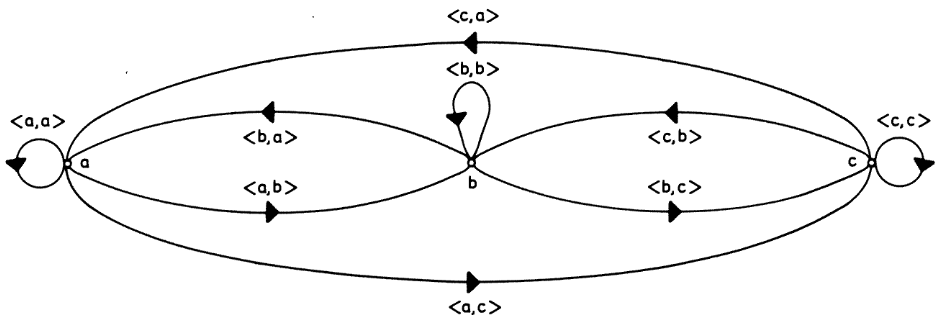
\includegraphics[width=1\textwidth]{img/Figura5-4.png}
		\\ \scriptsize Fig. 5.4. El gráfico de transición o de Moore para un elemento de tres estados.
	\end{center}

	Suponemos a continuación que la composición de ciertos eventos es posible,
	mientras que la de otros no lo es. Por ejemplo, el evento $e_4 = \langle a, b \rangle$ puede ir seguido
	del evento $e_5 = \langle b, c \rangle$, y el evento complejo puede considerarse como una
	descomposición del evento $e_6 = \langle a, c \rangle$. Para simbolizar la composición de
	eventos, utilizamos el asterisco * y escribimos: $e_4 * e_5 = e_6$ o, explícitamente,
	$\langle a, b \rangle * \langle b, c \rangle = \langle a, c \rangle$. (Es decir, los estados
	intermedios no aparecen en el cambio neto: se absorben). Por otro lado, el evento complejo
	$\langle b, c \rangle * \langle a, b \rangle$, que es el inverso del anterior, no se produce,
	por lo que queda sin definir. En otras palabras, para representar la combinación de
	eventos, introducimos una operación binaria (parcial) * en: $E(x)$. Si $e$ y $f$ están
	en $E(x)$, entonces $e * f = g$ es otro evento en $E(x)$ que consiste en que el evento $e$
	es seguido por el evento $f$, con la salvedad de que, en ciertos casos, la
	composición no está definida.
	
	Las posibles combinaciones binarias de eventos que ocurren en una cosa de tres estados
	se muestran en la siguiente tabla. Cada entrada de esta tabla de multiplicación
	muestra el cambio neto, no el proceso de cambio. Pero, por supuesto, el\

	\begin{center}
			\setlength{\tabcolsep}{3pt}
			\footnotesize \begin{tabular}{c|ccccccccc}
				* & $\langle a,a \rangle$ & $\langle a,b \rangle$ & $\langle a,c \rangle$ & $\langle b,a \rangle$ & $\langle b,b \rangle$ & $\langle b,c \rangle$ & $\langle c,a \rangle$ & $\langle c,b \rangle$ & $\langle c,c \rangle$ \\
				\hline
				$\langle a,a \rangle$ & $\langle a,a \rangle$ & $\langle a,b \rangle$ & $\langle a,c \rangle$ & & & & & & \\
				$\langle a,b \rangle$ &  &  &  & $\langle a,a \rangle$ & $\langle a,b \rangle$ & $\langle a,c \rangle$ & & & \\
				$\langle a,c \rangle$ &  &  &  &  &  &  & $\langle a,a \rangle$ & $\langle a,b \rangle$ & $\langle a,c \rangle$ \\
				$\langle b,a \rangle$ & $\langle b,a \rangle$ & $\langle b,b \rangle$ & $\langle b,c \rangle$ & & & & & & \\
				$\langle b,b \rangle$ &  & & & $\langle b,a \rangle$ & $\langle b,b \rangle$ & $\langle b,c \rangle$ & & & \\
				$\langle b,c \rangle$ &  & & & & & & $\langle b,a \rangle$ & $\langle b,b \rangle$ & $\langle b,c \rangle$ \\
				$\langle c,a \rangle$ & $\langle c,a \rangle$ & $\langle c,b \rangle$ & $\langle c,c \rangle$ & & & & & & \\
				$\langle c,b \rangle$ &  & & & $\langle c,a \rangle$ & $\langle c,b \rangle$ & $\langle c,c \rangle$ & & & \\
				$\langle c,c \rangle$ &  &  & & & & & $\langle c,a \rangle$ & $\langle c,b \rangle$ & $\langle c,c \rangle$ \\
			\end{tabular}
	\end{center}

	\noindent La tabla nos permite analizar ciertos eventos como procesos, es decir, secuencias de eventos elementales.
	De esta tabla se desprenden claramente una serie de regularidades. Suponemos
	que son válidas para todos los espacios de eventos y las resumimos en

	\bigskip

	\noindent DEFINICIÓN 5.4 Sea $S(x) \neq \varnothing$ un espacio de estado para una cosa $x$ y sea
	$E(x)=S(x) \times S(x)$. El triple $\mathscr{E} =(S(x),E(x), *)$, donde $*$ es una operación binaria parcial
	(no definida en todas partes) en $E(x)$ tal que, para todos los
	$a, b, c, d$ en $S(x)$,

	\[
	\langle a, b \rangle * \langle c, d \rangle =
	\begin{cases}
	\langle a, d \rangle \: \text{si } b = c \\
	\text{no definido} \: \text{si } b \neq c,
	\end{cases}
	\]

	\noindent Es el espacio de eventos de $x$ asociado con $S(x)$ si y solo si
	\begin{enumerate}[label=(\roman*), itemsep=0pt, parsep=0pt]
		\item  cada elemento de $E(x)$ representa un cambio concebible de (o evento en) la cosa $x$;
		\item para cualquier $e, f \in E(x)$, $e * f$ representa el evento que consiste en que
		el evento $e$ se compone con el evento $f$ en el orden indicado;
		\item para cualquier $s \in S(x)$, $(s, s) \in E(x)$ representa el evento de identidad 
		(o no evento) en $s$, es decir, la permanencia de $x$ en el estado $s$.
		\item Una consecuencia inmediata es que cada evento concebible $(s, s')$,
		donde $s, s' \in S(x)$, tiene un recíproco único, es decir, $\langle s', s \rangle$. (Lo que solo sirve
		para demostrar que $E(x)$ es la totalidad de los eventos concebibles, no de los realmente
		posibles). Otra consecuencia es
	\end{enumerate}

	\noindent COROLARIO 5.3 Para cada estado $s \in S(x)$ existe un evento de identidad
	$i_s = \langle s, s \rangle$ tal que, para cada $e \in E(x)$ para el que $*$ está definido, $e * i_s =
	i_s * e = e$.

	En otras palabras, la estructura $\mathscr{E} = \langle S(x), E(x), * \rangle$ es una categoría con conjunto
	de objetos $S(x)$, conjunto de morfismos $E(x)$ y morfismos de identidad $i_s$ para todos
	$s \in S(x)$; la composición es $*$. El gráfico de transición de la figura 5.6 es una
	representación gráfica vívida de esta categoría en el caso en que $S(x)$ tiene
	solo tres miembros.

	Tenga en cuenta que en la categoría $\mathscr{E}$ se cumple lo siguiente: para cualquier par de objetos
	(estados) $s, s' \in S(x)$ existe exactamente un morfismo $s \to s'$, a saber $(s, s')$.
	Esto, a su vez, implica que cada morfismo en la categoría es un isomorfismo,
	es decir, el inverso de $(s, s')$ es el morfismo único $(s', s)$. Esto implica

	\bigskip

    \noindent COROLARIO 5.4 Sean $s, s' \in S(x)$ estados de $x$. Entonces
    \begin{itemize}
        \item[(i)] ningun evento que no sea un evento de identidad es inmediatamente repetible: $(s, s') * (s, s')$ no est\'a definido en $E(x)$;
        \item[(ii)] Si un evento es seguido por su inverso, entonces no se produce ningún cambio neto: $ \langle s, s' \rangle * \langle s', s \rangle = \langle s, s \rangle. $
    \end{itemize}

    De la Definición 5.4 se desprende que los estados 
    intermedios no aparecen en el resultado neto. Por lo tanto, los dos procesos
    \bigskip
    \begin{center}
        \begin{tikzpicture}[
            node distance=1.5cm and 2cm,
            every node/.style={circle, draw, minimum size=3mm, inner sep=2pt},
            every edge/.style={draw, -{Stealth[length=2mm]}},
        ]
            % Colocar los nodos
            \node (a) {a};
            \node (s) [above right=of a] {s};
            \node (t) [below right=of a] {t};
            \node (b) [below right=of s] {b};

            % Dibujar las flechas (aristas)
            \path (a) edge (s);
            \path (s) edge (b);
            \path (a) edge (t);
            \path (t) edge (b);
        \end{tikzpicture}
    \end{center}
    \bigskip

    \noindent son equivalentes en que $\langle a, s \rangle * \langle s, b \rangle = \langle a, t \rangle * \langle t, b \rangle = \langle a, b \rangle$. Por lo tanto, podemos hacer

    \bigskip

    \noindent DEFINICIÓN 5.5 Dos eventos complejos (procesos) en un espacio de eventos dado son equivalentes si tienen el mismo resultado [es decir, si relacionan los mismos estados inicial y final].
    Por lo tanto, cada evento complejo puede interpretarse como una clase de equivalencia de procesos, es decir, el conjunto de todos los procesos con los mismos puntos finales (estados).
    Concluimos esta sección destacando dos nociones que han surgido tácitamente en la sección anterior y que serán de capital importancia en la siguiente: las de proceso y precedencia.
    DEFINICIÓN 5.6 Un evento complejo [es decir, uno formado por la composición de dos o más eventos] se denomina proceso.

    \bigskip

    \noindent DEFINICIÓN 5.7 Sea $(e)$ y $(e')$ dos eventos en un espacio de eventos dado (es decir, $(e,e')\in E(x)$ para algún elemento $(x)$), tales que $(e)$ y $(e')$ se componen para formar un tercer evento $(e'') = (e)\ast (e')$. 
    Entonces se dice que $(e)$ precede a $(e')$ con respecto al marco de referencia involucrado en $(E(x))$. Formalmente,
    \[
    \text{Si } e,e'\in E(x)\quad\text{entonces}\quad
    e\prec e'\overset{\mathrm{df}}{=} e\ast e'\in E(x).
    \]

    Por lo tanto, para que un evento se repita, la cosa debe primero regresar al estado inicial, ya sea a través del 
    evento converso (cuando sea posible) o a través de eventos intermedios, como en el caso de $\langle s, s' \rangle * \langle s', s'' \rangle * \langle s'', s \rangle = \langle s, s \rangle$. 
    De la Definición 5.4 se sigue que los estados intermedios no aparecen en el resultado neto. Así, los dos procesos
\end{justifying}
